\documentclass[aspectratio=169]{beamer}
\usepackage[spanish]{babel} % Define el idioma del documento
\usepackage{listings}
\usepackage{tikz}
\usetikzlibrary{positioning}
\usepackage{hyperref} % Utilizado para crear hipervínculos en el documento
\hypersetup{
	colorlinks=true,
	linkcolor=blue,
	filecolor=magenta,
	urlcolor=cyan,
}

\lstset{%
  frame            = tb,    % draw frame at top and bottom of code block
  tabsize          = 2,     % tab space width
  framesep         = 3pt,   % expand outward
  framerule        = 0.4pt, % expand outward 
  commentstyle     = \color{Green},      % comment color
  keywordstyle     = \color{blue},       % keyword color
  stringstyle      = \color{DarkRed},    % string color
  backgroundcolor  = \color{lightgray}, % backgroundcolor color
  showstringspaces = false,              % do not mark spaces in strings
  basicstyle=\scriptsize\ttfamily,
}

\usetheme{unad}

\title{Preparación de Documentos Técnicos Usando \LaTeX}
\author{Gerardo Becerra, Ph.D.}
\institute{UNAD}
\date{Febrero 26 de 2022}
\institute{Escuela de Ciencias Básicas, Tecnología e Ingeniería}
\city{Bogotá D.C.}

\usebackgroundtemplate%
{%
    
\includegraphics[width=\paperwidth,height=\paperheight]{img/content_background.jpg}%
}

\setbeamertemplate{caption}[numbered]

\AtBeginSection[]
{
	\begin{frame}<beamer>
		\frametitle{Agenda de la Presentación}
		\tableofcontents[currentsection]
	\end{frame}
}


\begin{document}

% Diapositiva de título
{\usebackgroundtemplate{
	
\includegraphics[width=\paperwidth]{img/cover_background.jpg}}%
	\frame{\titlepage}
}


\begin{frame}
	\frametitle{Agenda de la Presentación}
	\tableofcontents
\end{frame}

% Aquí inician los contenidos de la presentación
\section{Introducción al sistema \LaTeX}
\begin{frame}[t]\frametitle{¿Qué es \LaTeX?}
	\begin{itemize}
		\item Es un lenguaje creado por \href{https://en.wikipedia.org/wiki/Donald_Knuth}{Donald Knuth} y luego extendido por \href{https://en.wikipedia.org/wiki/Leslie_Lamport}{Leslie Lamport} para crear documentos atractivos y consistentes.
		\pause
		\item Es un lenguaje tipográfico y de marcado (markup):
		\begin{itemize}
			\item Tipográfico: Reglas que definen la organización y presentación de los contenidos en un documento.
			\item Marcado: Reglas que definen los contenidos de un documento.
		\end{itemize}
		\pause
		\item Estos dos aspectos se manejan por separado (Una persona crea la plantilla y otra se encarga de producir los contenidos del documento).
	\end{itemize}
\end{frame}

\begin{frame}[t]\frametitle{¿Por qué usar \LaTeX?}
	\begin{itemize}
		\item Dos enfoques diferentes:
		\pause
		\begin{itemize}
			\item Sistemas \emph{What You See is What You Get} (WYSIWYG): Microsoft Word, Google Docs, LibreOffice, etc. $\longrightarrow$ A medida que se va editando el documento se  va observando la apariencia que éste toma. 
			\pause
			\item \LaTeX\ $\longrightarrow$ Se utilizan comandos para describir los contenidos en un archivo de texto, y luego un programa se encarga de producir el documento.
		\end{itemize}
	\end{itemize}	
\end{frame}

\begin{frame}[t]\frametitle{¿Por qué usar \LaTeX?}
	\begin{itemize}
		\item Ventajas:
		\pause
		\begin{itemize}
			\item El autor se puede concentrar únicamente en la estructura y contenidos del documento. \LaTeX\ se encarga de aplicar las reglas tipográficas para producir un documento consistente.
			\pause
			\item En \LaTeX\ es fácil reproducir la estructura de un documento.
			\pause
			\item Manejo automático de índices, pies de página, citaciones y referencias.
			\pause
			\item Las fórmulas matemáticas se pueden preparar fácilmente.
			\pause
			\item El documento de origen es texto plano
			\begin{itemize}
			 	\item Lectura en cualquier sistema
			 	\item Generación automática de contenidos
			 	\item Control de versiones
			 \end{itemize}
			\pause
			\item La preparación de artículos para revistas y conferencias internacionales se realiza usando plantillas de \LaTeX.
			\pause
			\item ¡Es gratuito!
		\end{itemize}
	\end{itemize}
\end{frame}

\begin{frame}[t]\frametitle{¿Cómo obtener \LaTeX?}
	\begin{itemize}
		\item Para empezar, ¡no se requiere instalar nada! $\longrightarrow$ Editor en línea: \href{https://www.overleaf.com}{Overleaf}.
		\pause
		\item Para trabajar fuera de línea, se descarga y se instala una distribución de \LaTeX:
		\begin{itemize}
			\item \href{http://www.tug.org/texlive/}{TeX Live}: Distribución multiplataforma.
			\item \href{http://www.miktex.org/}{MiKTeX}: Distribución multiplataforma.
			\item \href{http://www.tug.org/mactex/}{MacTeX}: Distribución para Mac OS, basada en TeX Live.
		\end{itemize}
		\pause
		\item Para preparar los documentos se requiere un \href{https://en.wikipedia.org/wiki/Comparison_of_TeX_editors}{editor de texto}.
		\pause
		\item Para usar funcionalidades específicas, se pueden instalar \href{https://www.ctan.org/}{paquetes adicionales}.
	\end{itemize}
\end{frame}

\section{Fundamentos de \LaTeX}
\begin{frame}[fragile]\frametitle{La Sintaxis de \LaTeX}
\begin{columns}
	\begin{column}{0.5\textwidth}
		Para crear un documento se puede utilizar cualquier editor de texto. A continuación se encuentra un ejemplo mínimo:
		\begin{lstlisting}
\documentclass{article}
% Preambulo
\begin{document}
	Contenidos del documento...
\end{document}	
		\end{lstlisting}
	\end{column}
	\pause
	\begin{column}{0.5\textwidth}
		El documento obtenido será el siguiente:
		\begin{figure}
			\centering
			
\includegraphics[width=\textwidth]{img/ejemplo_minimo.png}
		\end{figure}
	\end{column}
\end{columns}
\end{frame}

\begin{frame}[fragile]\frametitle{Espacios en Blanco}
	\begin{columns}
		\begin{column}{0.5\textwidth}
			\begin{itemize}
				\item El compilador de \LaTeX\ normaliza los espacios en blanco. Varios caracteres consecutivos de [espacio] y [tabulador] son tratados como uno sólo.
				\pause
				\item Un salto de línea sencillo [Enter] también es tratado como un espacio en blanco.
				\pause
				\item Dos saltos de línea definen un nuevo párrafo.
				\pause
			\end{itemize}
		\end{column}
		\begin{column}{0.5\textwidth}
			\begin{lstlisting}
No importa si se introducen
uno o mas            espacios
despues de una	palabra.

Una linea vacia siempre
inicia un nuevo parrafo.
			\end{lstlisting}
			\begin{figure}
				\centering
				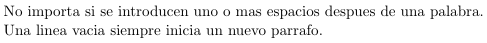
\includegraphics[width=\textwidth]{img/espacio_blanco.png}
			\end{figure}
		\end{column}
	\end{columns}	
\end{frame}

\begin{frame}[fragile]\frametitle{Caracteres Reservados}
	\begin{itemize}
		\item Los siguientes símbolos son de uso reservado y si se introducen directamente en el texto pueden generar errores: \#\ \$\ \%\ \^\ \&\ \_\ \{\ \}\ \~\ \textbackslash{}.
		\pause
		\item Para utilizarlos dentro del texto se adiciona el caracter \textbackslash{} de la siguiente manera:
		\begin{lstlisting}
\# \$ \% \^ \& \_ \{ \} \~ \textbackslash{}
		\end{lstlisting}
	\end{itemize}
\end{frame}

\begin{frame}[fragile]\frametitle{Entornos de \LaTeX (Environments)}
	\begin{itemize}
		\item Son estructuras que definen las características locales de los contenidos en el documento.
		\pause
		\item Su sintaxis se define de la siguiente manera:
		\begin{lstlisting}
\begin{nombreentorno}
	Texto o contenidos que van a ser influenciados
\end{nombreentorno}
		\end{lstlisting}
	\end{itemize}
\end{frame}

\begin{frame}[fragile]\frametitle{Comandos de \LaTeX}
	\begin{itemize}
		\item Los comandos inician con el caracter backslash \textbackslash{} y continúan con el nombre.
		\pause
		\item Algunos comandos requieren argumentos obligatorios que se debe dar dentro de llaves \{\ \}.
		\pause
		\item Algunos comandos poseen argumentos opcionales que se debe dar dentro de corchetes [\ ].
		\pause
		\item La sintáxis general es:
		\begin{lstlisting}
\nombrecomando[opcion1,opcion2,...]{argum1}{argum2}...
		\end{lstlisting}
	\end{itemize}
\end{frame}

\begin{frame}[fragile]\frametitle{Comentarios}
	\begin{itemize}
		\item El caracter \% se utiliza para representar comentarios dentro del archivo de texto.
		\pause
		\item \LaTeX\ ignora el contenido que se encuentra después del caracter \% y no lo incluye en el documento preparado.
		\pause
		\item \LaTeX\ también ignora el salto de línea y todo el espacio en blanco al inicio de la siguiente línea.
	\end{itemize}
	\pause
	\begin{columns}
		\begin{column}{0.5\textwidth}
			\begin{lstlisting}
% Este texto no es mostrado
% Este tampoco
Este texto si es visible

Otra linea de % comentario
       contenido
			\end{lstlisting}
		\end{column}
		\begin{column}{0.5\textwidth}
			\begin{figure}
				\centering
				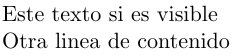
\includegraphics[width=4cm]{img/comentarios.png}
			\end{figure}
		\end{column}
	\end{columns}
\end{frame}

\begin{frame}[t]\frametitle{Generar el Documento}
	\begin{itemize}
		\item Los archivos de texto fuente de \LaTeX\ se guardan con la extensión \texttt{tex} (p.ej. \texttt{hola.tex}
		\pause
		\item Para compilar el archivo de texto fuente se utiliza el comando \texttt{latex} junto con el nombre del archivo (p.ej. \texttt{latex hola}. Éste comando producirá un archivo con extensión \texttt{dvi} (p.ej. \texttt{hola.dvi}).
		\pause
		\item Luego, para generar el archivo final en formato \texttt{pdf} se utiliza el comando \texttt{pdflatex} (p.ej. \texttt{pdflatex hola}).
		\pause
		\item Si se utiliza un editor de texto estos comandos se ejecutan de manera automática.
		\pause
		\item También existen sistemas para realizar la compilación en un sólo paso. Por ejemplo \texttt{latexmk -pdf hola.tex}.
		\pause
		\item El proceso de compilación produce algunos archivos auxiliares (\texttt{aux}, \texttt{log}, \texttt{fls}, \texttt{nav}, etc).
	\end{itemize}
\end{frame}


\section{Elementos Generales del Lenguaje \LaTeX}
\begin{frame}[t]\frametitle{Estructura General del Documento}
	\begin{itemize}
		\item Para comunicar mejor nuestras ideas, nuestros textos deben tener una estructura lógica.
		\pause
		\item \LaTeX\ requiere que el autor indique la estructura lógica del contenido para preparar el documento de acuerdo a las reglas de \emph{typesetting}.
		\pause
		\item \LaTeX\ permite utilizar estructuras jerárquicas tales como capítulos, secciones, subsecciones y parágrafos.
	\end{itemize}
\end{frame}

\begin{frame}[fragile]\frametitle{Estructura General del Documento}
    
\begin{lstlisting}[numbers = none, escapechar = !,
    basicstyle = \ttfamily\bfseries, linewidth = .6\linewidth] 
 \documentclass[options]{class} !\tikz[remember picture] \node [] (a) {};!

	\includepackage{package1} !\tikz[remember picture] \node [] (b){};!           
	\includepackage{package2}
    
\begin{document} !\tikz[remember picture] \node [] (c){};! 
	...	
	Contenidos !\tikz[remember picture] \node [] (d){};!  
	...
\end{document} !\tikz[remember picture] \node [] (e){};!
\end{lstlisting}
\begin{tikzpicture}[remember picture, overlay,
    every edge/.append style = { ->, thick, >=stealth,
                                  gray, dashed, line width = 1pt },
    every node/.append style = { align = center, minimum height = 10pt,
                                 font = \bfseries, fill= green!20},
                  text width = 5cm ]
  \node [right = 1.0cm of a]  (A) {Clase del documento};
  \node [right = 2.0cm of b]  (B) {Preámbulo};
  \node [right = 4.7cm of c]  (C) {Inicio entorno documento};
  \node [right = 5.6cm of d]  (D) {Contenidos del documento};  
  \node [right = 5.1cm of e]  (E) {Fin entorno documento};  
  \draw (A.west) edge (a.east);
  \draw (B.west) edge (b.east) ;
  \draw (C.west) edge (c.east) ;  
  \draw (D.west) edge (d.east) ;
  \draw (E.west) edge (e.east) ;
\end{tikzpicture}
\end{frame}

\begin{frame}[t]\frametitle{Clases de Documentos}
	\centering
	\begin{tabular}{ll}
		\hline
		\textbf{Clase} & \textbf{Descripción}\\
		\hline
		\texttt{article} & Artículos de revista, reportes, documentación, etc\\
		\texttt{IEEEtran} & Artículos con formato IEEE Transactions\\
		\texttt{report} & Reportes largos con varios capítulos, libros cortos, tesis\\
		\texttt{book} & Libros\\
		\texttt{letter} & Cartas\\
		\texttt{beamer} & Presentaciones\\
		\hline
	\end{tabular}
\end{frame}

\begin{frame}[t]\frametitle{Ejercicio 1}
	\begin{enumerate}
	 	\item Crea un documento usando la clase \texttt{article} donde se incluya título, autor y fecha. Configura el papel en tamaño carta. Utiliza el paquete \texttt{lipsum} para generar textos genéricos.
		\pause
	 	\item Modifica el documento anterior para configurar el papel en tamaño A4 y organizar el texto en doble columna. Cambia el tamaño base del tipo de letra a 12 puntos.
	\end{enumerate} 
\end{frame}

\begin{frame}[fragile]\frametitle{Resumen del Documento}
	En muchas situaciones, se requiere introducir un resumen (abstract) al inicio del documento. Para hacerlo se usa el entorno \texttt{abstract}:
	\begin{lstlisting}
\begin{abstract}
	Escribe aqui tu resumen...
\end{abstract}
	\end{lstlisting}
\end{frame}

\begin{frame}[t]\frametitle{Secciones del Documento}
	La estructura lógica de un documento puede dividirse en una jerarquía de partes, capítulos, secciones, parágrafos, etc. En la siguiente tabla se muestran los diferentes niveles y los comandos a utilizar:\\
	\begin{table}
		\centering
		\begin{tabular}{lc}
			\hline
			\textbf{Comando} & \textbf{Nivel}\\
			\hline
			\texttt{\textbackslash{}part\{parte\}} & -1\\
			\texttt{\textbackslash{}chapter\{capítulo\}} & 0\\
			\texttt{\textbackslash{}section\{sección\}} & 1\\
			\texttt{\textbackslash{}subsection\{subsección\}} & 2\\
			\texttt{\textbackslash{}subsubsection\{subsubsección\}} & 3\\
			\texttt{\textbackslash{}paragraph\{parágrafo\}} & 4\\
			\texttt{\textbackslash{}subparagraph\{subparágrafo\}} & 5\\
			\hline
		\end{tabular}
	\end{table}
\end{frame}


\begin{frame}[t]\frametitle{Ejercicio 2}
	\begin{enumerate}
	 	\item Crea un artículo que incluya los siguientes elementos: título, autor, fecha, resumen, tabla de contenido y contenido. Organiza el contenido en las secciones introducción, metodología, resultados y conclusiones. Utiliza el paquete \texttt{lipsum} para generar los textos.
		\pause
	 	\item Crea un libro que tenga 3 capítulos: introducción, desarrollo y conclusión. Cada capítulo debe tener 3 secciones. El libro debe tener una portada con el título, autor y fecha. También debe incluir la tabla de contenido.
	\end{enumerate} 
\end{frame}

\begin{frame}[t]\frametitle{Gestión de Referencias Bibliográficas}
	\begin{itemize}
		\item La mayoría de documentos técnicos se basan en otras fuentes de información para desarrollar sus contenidos.
		\pause
		\item Es necesario incluir referencias a dichas fuentes.
		\pause
		\item \LaTeX\ permite insertar fácilmente estas referencias.
		\pause
		\item Para manejar las referencias es recomendable utilizar el paquete \texttt{biblatex}
	\end{itemize}
\end{frame}

\begin{frame}[t]\frametitle{Gestión de Referencias Bibliográficas}
	Los comandos básicos de \texttt{biblatex} a utilizar son:
	\begin{itemize}
		\item \texttt{\textbackslash{}usepackage\{biblatex\}}: Importa el paquete \texttt{biblatex}.
		\pause
		\item \texttt{\textbackslash{}addbibresource\{referencias.bib\}}: Importa el archivo \texttt{referencias.bib} donde se encuentra la información bibliográfica de las fuentes de información.
		\pause
		\item \texttt{\textbackslash{}cite\{nombreref\}}: Inserta una cita dentro del documento, usando la referencia \texttt{nombreref}.
		\pause
		\item \texttt{\textbackslash{}printbibliography:} Imprime la lista de referencias citadas dentro del texto.
	\end{itemize}
\end{frame}

\begin{frame}[fragile]\frametitle{Biblatex - Ejemplo de Uso}
	Definimos el archivo \texttt{referencias.bib}:
	\begin{lstlisting}
@book{lamport1994latex,
	title={LATEX: A Document Preparation System: User's Guide and Reference Manual},
	author={Lamport, L. and Bibby, D. and Pearson Education},
	isbn={9780201529838},
	lccn={93039691},
	series={Addison-Wesley Series on Tools},
	url={https://books.google.com.co/books?id=khVUAAAAMAAJ},
	year={1994},
	publisher={Addison-Wesley}
}
	\end{lstlisting} 
\end{frame}

\begin{frame}[fragile]\frametitle{Biblatex - Ejemplo de Uso}
	Ahora definimos el archivo principal \texttt{main.tex}:
	\begin{lstlisting}
\documentclass{article}

\usepackage{biblatex}
\addbibresource{referencias.bib}

\begin{document}
	Leslie Lamport ha publicado \cite{lamport1994latex} una
	introduccion al	lenguaje \LaTeX\ para la preparacion de
	documentos tecnicos.

	\printbibliography
\end{document}
	\end{lstlisting} 
\end{frame}

\begin{frame}[t]\frametitle{Biblatex - Ejemplo de Uso}
	Al compilar el archivo principal, el resultado obtenido es el siguiente:
	\begin{figure}
		\centering
		
\includegraphics[width=12cm]{img/bibliografia.png}
	\end{figure}
\end{frame}

\begin{frame}[fragile]\frametitle{Ejercicio 3}
	\begin{enumerate}
		\item Crea un archivo \texttt{referencias.bib} con la información de libros y artículos disponible en diferentes bases de datos: \href{https://books.google.com}{Google Books}, \href{https://ieeexplore.ieee.org/}{IEEE Xplore}, \href{https://www.sciencedirect.com/}{ScienceDirect}.
		\pause
		\item Usando el artículo creado en el ejercicio 2-1, agrega los comandos para cargar el paquete \texttt{biblatex}, importar el archivo de referencias, incluir varias citas dentro del texto e imprimir las referencias al final del documento.
		\pause
		\item Agrega el siguiente comando al preámbulo. ¿Qué diferencias encuentras?
		\begin{lstlisting}
	\usepackage[spanish]{babel}
		\end{lstlisting}
		\pause
		\item Utiliza la opción \texttt{style=apa} al importar \texttt{biblatex}. ¿Cómo cambian las citaciones?
	\end{enumerate}
\end{frame}

\begin{frame}[fragile]\frametitle{Listas en \LaTeX}
	\begin{columns}
		\begin{column}{0.5\textwidth}
			\begin{itemize}
				\item En documentos técnicos, es común utilizar listas para presentar la información de manera clara y concisa.
				\pause
				\item \LaTeX\ incluye tres tipos de lista:
				\begin{enumerate}
					\item \texttt{itemize}: lista simple.
					\item \texttt{enumerate}: lista numerada.
					\item \texttt{description}: lista descriptiva.
				\end{enumerate}
				\pause
			\end{itemize}
		\end{column}
		\begin{column}{0.5\textwidth}
			\begin{itemize}
				\item Todas las listas tienen el siguiente formato:
				\begin{lstlisting}
\begin{tipo_lista}
	\item Primer elemento
	\item Segundo elemento
	\item Tercer elemento
\end{tipo_lista}
				\end{lstlisting}
			\end{itemize}
		\end{column}
	\end{columns}
\end{frame}

\begin{frame}[fragile]\frametitle{Listas en \LaTeX\ - Ejemplos}
	\begin{columns}
		\begin{column}{0.33\textwidth}
			\begin{figure}
				\centering
				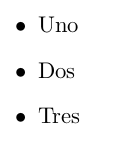
\includegraphics[width=2cm]{img/lista1.png}
			\end{figure}
			\begin{lstlisting}
\begin{itemize}
	\item Uno 
	\item Dos 
	\item Tres
\end{itemize}
			\end{lstlisting}
		\end{column}
		\pause
		\begin{column}{0.33\textwidth}
			\begin{figure}
				\centering
				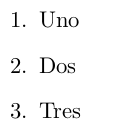
\includegraphics[width=2.1cm]{img/lista2.png}
			\end{figure}
			\begin{lstlisting}
\begin{enumerate}
	\item Uno
	\item Dos
	\item Tres
\end{enumerate}
			\end{lstlisting}
		\end{column}
		\pause
		\begin{column}{0.33\textwidth}
			\begin{figure}
				\centering
				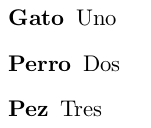
\includegraphics[width=2.3cm]{img/lista3.png}
			\end{figure}
			\begin{lstlisting}
\begin{description}
	\item[Gato] Uno
	\item[Perro] Dos
	\item[Pez] Tres
\end{description}
			\end{lstlisting}
		\end{column}
	\end{columns}
\end{frame}

\begin{frame}[fragile]\frametitle{Tablas en \LaTeX}
\begin{columns}
	\begin{column}{0.5\textwidth}
		\begin{itemize}
			\item En documentos técnicos es muy común utilizar tablas para presentar información.
			\pause
			\item \LaTeX\ ofrece el entorno \texttt{tabular} para organizar la información en forma de tablas.
			\pause
			\item El formato básico del entorno \texttt{tabular} es el siguiente:
			\begin{lstlisting}
\begin{tabular}{params}
	Datos tabulares
\end{tabular}
			\end{lstlisting}
		\end{itemize}
	\end{column}
	\begin{column}{0.5\textwidth}
		\pause
		\begin{itemize}
			\item Parámetros:
			\begin{table}
				\centering
				\begin{tabular}{|l|l|}
					\hline
					l & alineación izquierda\\
					\hline
					c & alineación centrada\\
					\hline
					r & alineación derecha\\
					\hline
					| & línea vertical\\
					\hline
					|| & doble línea vertical\\
					\hline
				\end{tabular}
			\end{table}
			\pause
			\item Comandos en los datos tabulares:
			\vspace{-5mm}
			\begin{table}
				\centering
				\begin{tabular}{|l|l|}
					\hline
					\& & Separador de columnas\\
					\hline
					\textbackslash\textbackslash & Inicia nueva fila\\
					\hline
					\textbackslash{}\texttt{hline} & Línea horizontal\\
					\hline
					\textbackslash{}\texttt{cline}\{i-j\} & Línea horizontal parcial\\
					\hline
				\end{tabular}
			\end{table}
		\end{itemize}
	\end{column}
\end{columns}
\end{frame}

\begin{frame}[fragile]\frametitle{Tablas en \LaTeX\ - Ejemplo}
	\begin{columns}
		\begin{column}{0.5\textwidth}
			\begin{figure}
				\centering
				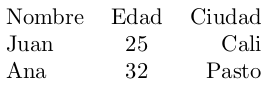
\includegraphics[width=5cm]{img/tabla1.png}
			\end{figure}
			\begin{lstlisting}
\begin{tabular}{lcr}
	Nombre & Edad & Ciudad\\
	Juan & 25 & Cali\\
	Ana & 32 & Pasto
\end{tabular}
			\end{lstlisting}
		\end{column}
		\pause
		\begin{column}{0.5\textwidth}
			\begin{figure}
				\centering
				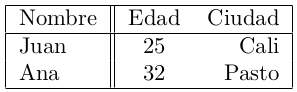
\includegraphics[width=5cm]{img/tabla2.png}
			\end{figure}
			\begin{lstlisting}
\begin{tabular}{|l||cr|}
	\hline
	Nombre & Edad & Ciudad\\
	\hline
	Juan & 25 & Cali\\
	Ana & 32 & Pasto\\
	\hline
\end{tabular}
			\end{lstlisting}
		\end{column}
	\end{columns}
\end{frame}

\begin{frame}[fragile]\frametitle{Incluir Gráficos en \LaTeX}
\begin{columns}
	\begin{column}{0.5\textwidth}
	\begin{itemize}
		\item Muchos documentos técnicos requieren incluir gráficos para presentar ideas, resultados, estadísticas, etc.
		\pause
		\item Es posible importar gráficos de mapas de bits (p.ej. \texttt{png}, \texttt{jpg}). Sin embargo idealmente es mejor trabajar con gráficos vectoriales (p.ej. \texttt{pdf}, \texttt{eps}).
		\pause
		\item El comando básico para incluir gráficos es el siguiente:
		\begin{lstlisting}
\includegraphics[params]{nombreimg}
		\end{lstlisting}
	\end{itemize}
	\end{column}	
	\pause
	\begin{column}{0.5\textwidth}
	\begin{itemize}
		\item Para documentos del tipo \texttt{article}, es necesario importar el paquete \texttt{graphicx}.
		\pause
		\item Algunos de los parámetros más utilizados son:
		\begin{table}
			\centering
			\begin{tabular}{|l|l|}
				\hline
				\texttt{width=x} & Ancho del gráfico\\
				\hline
				\texttt{height=x} & Alto del gráfico\\
				\hline
				\texttt{scale=x} & Escala del gráfico\\
				\hline
				\texttt{angle=x} & Ángulo del gráfico\\
				\hline
			\end{tabular}
		\end{table}
	\end{itemize}
	\end{column}	
\end{columns}
\end{frame}

\begin{frame}[fragile]\frametitle{Incluir Gráficos en \LaTeX\ - Ejemplos}
			\begin{figure}
				\centering
				
\includegraphics[width=3cm]{img/logo.png}
			\end{figure}
			\begin{lstlisting}

\includegraphics[width=2cm]{logo.png}
			\end{lstlisting}
			\pause
			\begin{figure}
				\centering
				
\includegraphics[width=\textwidth,height=1cm]{img/logo.png}
			\end{figure}
			\begin{lstlisting}

\includegraphics[width=\textwidth,height=1cm]{logo.png}
			\end{lstlisting}
\end{frame}

\begin{frame}[fragile]\frametitle{Incluir Gráficos en \LaTeX\ - Ejemplos}
			\vspace{-5mm}
			\begin{figure}
				\centering
				
\includegraphics[width=2cm,angle=45]{img/logo.png}
			\end{figure}
			\vspace{-5mm}
			\begin{lstlisting}

\includegraphics[width=2cm,angle=45]{logo.png}
			\end{lstlisting}
			\pause
			\begin{figure}
				\centering
				
\includegraphics[scale=0.02]{img/logo.png}
			\end{figure}
			\begin{lstlisting}

\includegraphics[scale=0.02]{logo.png}
			\end{lstlisting}
\end{frame}

\begin{frame}[fragile]\frametitle{Figuras y Leyendas en \LaTeX}
	\begin{columns}
		\begin{column}{0.4\textwidth}
			\begin{itemize}
				\item Las imágenes que hemos insertado usando el comando \texttt{\textbackslash{}includegraphics} quedan embebidos dentro del párrafo.
				\pause
				\item Para colocar las imágenes de manera separada al texto y poder hacer referencia a estas, se utiliza el entorno \texttt{figure}:
				\begin{lstlisting}
\begin{figure}[spec]
	... contenido ...
\end{figure}
				\end{lstlisting}
			\end{itemize}
		\end{column}
		\pause
		\begin{column}{0.6\textwidth}
	\begin{itemize}
		\item El parámetro \texttt{spec} es un especificador que controla la ubicación de la figura:
		\begin{figure}
			\centering
			\begin{tabular}{|c|l|}
				\hline
				\textbf{Especificador} & \textbf{Permiso}\\
				\hline
				\texttt{h} & Ubicar aquí la figura\\
				\hline
				\texttt{t} & Ubicar al inicio de la página\\
				\hline
				\texttt{b} & Ubicar al final de la página\\
				\hline
				\texttt{p} & Ubicar en una página propia\\
				\hline
				\texttt{!} & Anular los criterios internos\\
				\hline
			\end{tabular}
		\end{figure}
	\end{itemize}
		\end{column}
	\end{columns}
\end{frame}

\begin{frame}[fragile]\frametitle{Figuras y Leyendas en \LaTeX}
	\begin{itemize}
		\item Para incluir una leyenda en una figura se utiliza el comando \texttt{\textbackslash{}caption}:
		\begin{figure}
			
\includegraphics[width=2cm]{img/logo.png}
			\caption{Logotipo de la UNAD}
		\end{figure}
		\begin{lstlisting}
\begin{figure}
	
\includegraphics[width=2cm]{logo.png}
	\caption{Logotipo de la UNAD}
\end{figure}
		\end{lstlisting}
	\end{itemize}
\end{frame}

\begin{frame}[fragile]\frametitle{Figuras y Leyendas en \LaTeX}
	\begin{itemize}
		\item Para incluir una referencia a una figura dentro del texto primero se crea un rótulo usando el comando \texttt{\textbackslash{}label}:
		\begin{columns}
			\begin{column}{0.3\textwidth}
				\begin{figure}
					
\includegraphics[width=2cm]{img/logo.png}
					\caption{Logotipo de la UNAD}
					\label{fig:logo UNAD}
				\end{figure}
			\end{column}
			\begin{column}{0.7\textwidth}
				\begin{lstlisting}
\begin{figure}
	
\includegraphics[width=2cm]{logo.png}
	\caption{Logotipo de la UNAD}
	\label{fig:logo UNAD}
\end{figure}
				\end{lstlisting}
			\end{column}
		\end{columns}
		\pause
		\item Luego se incluye una referencia a la figura \ref{fig:logo UNAD} en el texto usando el comando \texttt{\textbackslash{}ref}:
		\begin{lstlisting}
\ref{fig:logo UNAD}
		\end{lstlisting}
	\end{itemize}
\end{frame}

\begin{frame}[fragile]\frametitle{Figuras y Leyendas en \LaTeX}
	\begin{columns}
		\begin{column}{0.5\textwidth}
			\begin{itemize}
				\item Para crear una tabla con leyenda, se utiliza el entorno \texttt{table}:
		\begin{lstlisting}
\begin{table}
	\begin{tabular}{|l||cr|}
		\hline
		Nombre & Edad & Ciudad\\
		\hline
		Juan & 25 & Cali\\
		Ana & 32 & Pasto\\
		\hline
	\end{tabular}
	\caption{Estudiantes del curso}
	\label{tab:estudiantes curso}
\end{table}
		\end{lstlisting}
			\end{itemize}
		\end{column}
		\pause
	\begin{column}{0.5\textwidth}
		\begin{table}
			\begin{tabular}{|l||cr|}
				\hline
				Nombre & Edad & Ciudad\\
				\hline
				Juan & 25 & Cali\\
				Ana & 32 & Pasto\\
				\hline
			\end{tabular}
			\caption{Estudiantes del curso}
			\label{tab:estudiantes curso}
		\end{table}
		\pause
		\vspace{-5mm}
		\begin{itemize}
			\item Al igual que en las figuras, el rótulo se puede utilizar para hacer referencia al cuadro \ref{tab:estudiantes curso}:
			\begin{lstlisting}
\ref{tab:estudiantes curso}
			\end{lstlisting}
			\pause
			\item Listas de figuras y tablas: \texttt{\textbackslash{}listoffigures}, \texttt{\textbackslash{}listoftables}.
		\end{itemize}
	\end{column}
	\end{columns}
\end{frame}

\begin{frame}[fragile]\frametitle{Notas de Pie de Página en \LaTeX}
	\begin{itemize}
		\item Crear una nota de pie de página es muy fácil.\footnote{Esta es una nota de pie de página.}
		\item Para crear una nota de pie de página se utiliza el comando \texttt{\textbackslash{}footnote\{texto\}}.
	\end{itemize}
\end{frame}

\begin{frame}[fragile]\frametitle{Expresiones Matemáticas en \LaTeX}
\begin{columns}
	\begin{column}{0.5\textwidth}
	\begin{itemize}
		\item Una de las principales ventajas de \LaTeX\ es la facilidad para preparar expresiones matemáticas.
		\pause
		\item Existen diferentes entornos para preparar expresiones matemáticas:
		\begin{itemize}
			\item \texttt{\$...\$}: Expresión matemática embebida (\emph{en línea}) en el texto.
			\item \texttt{equation}: Expresión matemática separada del texto (\emph{flotante}).
		\end{itemize}
		\pause
		\item Para producir la expresión $x^2 + y^2 = 1$ en línea:
		\begin{lstlisting}
$x^2 + y^2 = 1$
		\end{lstlisting}
	\end{itemize}
	\end{column}
	\pause
	\begin{column}{0.5\textwidth}
	\begin{itemize}
		\item La ecuación \eqref{eq:ecuacion1} es una expresión flotante:
		\begin{equation}
			\sin^2\theta + \cos^2\theta = 1
			\label{eq:ecuacion1}
		\end{equation}
		\begin{lstlisting}
\begin{equation}
	\sin^2\theta + \cos^2\theta = 1
	\label{eq:ecuacion1}
\end{equation}
		\end{lstlisting}
		\pause
		Para referenciarla se usa \texttt{\textbackslash{}eqref\{eq:ecuacion1\}}
		\item Se requiere el paquete \texttt{amsmath} o \texttt{mathtools}.
	\end{itemize}
	\end{column}
\end{columns}
\end{frame}

\begin{frame}[fragile]\frametitle{Operadores Matemáticos en \LaTeX}
	\begin{itemize}
		\item \textbf{Categoría}: Funciones Trigonométricas.
		\item \textbf{Operadores}: \texttt{\textbackslash{}sin}, \texttt{\textbackslash{}cos}, \texttt{\textbackslash{}tan}, ...
		\item \textbf{Código}:
		\begin{lstlisting}
\begin{equation*}
	\cos(0) = 1
\end{equation*}
		\end{lstlisting}
		\item \textbf{Resultado}:
		\begin{equation*}
			\cos(0) = 1
		\end{equation*}
	\end{itemize}
\end{frame}

\begin{frame}[fragile]\frametitle{Operadores Matemáticos en \LaTeX}
	\begin{itemize}
		\item \textbf{Categoría}: Potencias, Indices
		\item \textbf{Operadores}: \texttt{\^}, \texttt{\_}
		\item \textbf{Código}:
		\begin{lstlisting}
\begin{equation*}
	k_{n+1}=n^{10}+k_n^2
\end{equation*}
		\end{lstlisting}
		\item \textbf{Resultado}:
		\begin{equation*}
			k_{n+1}=n^{10}+k_n^2
		\end{equation*}
	\end{itemize}
\end{frame}

\begin{frame}[fragile]\frametitle{Operadores Matemáticos en \LaTeX}
	\begin{itemize}
		\item \textbf{Categoría}: Fracciones
		\item \textbf{Operadores}: \texttt{\textbackslash{}frac}
		\item \textbf{Código}:
		\begin{lstlisting}
\begin{equation*}
			\frac{n!}{k!(n-k)!}
\end{equation*}
		\end{lstlisting}
		\item \textbf{Resultado}:
		\begin{equation*}
			\frac{n!}{k!(n-k)!}
		\end{equation*}
	\end{itemize}
\end{frame}

\begin{frame}[fragile]\frametitle{Operadores Matemáticos en \LaTeX}
	\begin{itemize}
		\item \textbf{Categoría}: Raíces
		\item \textbf{Operadores}: \texttt{\textbackslash{}sqrt}
		\item \textbf{Código}:
		\begin{lstlisting}
\begin{equation*}
	\sqrt[n]{1+x^2}
\end{equation*}
		\end{lstlisting}
		\item \textbf{Resultado}:
		\begin{equation*}
			\sqrt[n]{1+x^2}
		\end{equation*}
	\end{itemize}
\end{frame}

\begin{frame}[fragile]\frametitle{Operadores Matemáticos en \LaTeX}
	\begin{itemize}
		\item \textbf{Categoría}: Sumas
		\item \textbf{Operadores}: \texttt{\textbackslash{}sum}
		\item \textbf{Código}:
		\begin{lstlisting}
\begin{equation*}
	\sum_{i=1}^{10} t_i
\end{equation*}
		\end{lstlisting}
		\item \textbf{Resultado}:
		\begin{equation*}
			\sum_{i=1}^{10} t_i
		\end{equation*}
	\end{itemize}
\end{frame}

\begin{frame}[fragile]\frametitle{Operadores Matemáticos en \LaTeX}
	\begin{itemize}
		\item \textbf{Categoría}: Integrales
		\item \textbf{Operadores}: \texttt{\textbackslash{}int}
		\item \textbf{Código}:
		\begin{lstlisting}
\begin{equation*}
	\int_0^\infty \mathrm{e}^{-x}\,\mathrm{d}x
\end{equation*}
		\end{lstlisting}
		\item \textbf{Resultado}:
		\begin{equation*}
			\int_0^\infty \mathrm{e}^{-x}\,\mathrm{d}x
		\end{equation*}
	\end{itemize}
\end{frame}

\begin{frame}[fragile]\frametitle{Operadores Matemáticos en \LaTeX}
	\begin{itemize}
		\item \textbf{Categoría}: Corchetes, llaves y delimitadores
		\item \textbf{Operadores}: \texttt{(, ), [, ], \{, \}, \textbackslash{}langle, \textbackslash{}rangle, \textbackslash{}lfloor, \textbackslash{}rfloor, \textbackslash{}lceil, \textbackslash{}rceil, \textbackslash{}ulcorner, \textbackslash{}urcorner}
		\item \textbf{Código}:
		\begin{lstlisting}
\begin{equation*}
	(\frac{x^2}{y^3}), \left(\frac{x^2}{y^3}\right), 
	\frac{\mathrm d}{\mathrm d x} \big( k g(x) \big)
\end{equation*}
		\end{lstlisting}
		\item \textbf{Resultado}:
		\begin{equation*}
			(\frac{x^2}{y^3}), \left(\frac{x^2}{y^3}\right),
			\frac{\mathrm d}{\mathrm d x} \big( k g(x) \big)
		\end{equation*}
	\end{itemize}
\end{frame}

\begin{frame}[fragile]\frametitle{Operadores Matemáticos en \LaTeX}
	\begin{columns}
		\begin{column}{0.39\textwidth}
			\begin{itemize}
				\item \textbf{Categoría}: Matrices y arreglos
				\item \textbf{Entornos}: \texttt{matrix, pmatrix, bmatrix, Bmatrix, vmatrix, Vmatrix}.
				\item \textbf{Resultado}:
				\begin{equation*}
					A_{m,n} = 
					\begin{pmatrix}
						a_{1,1} & a_{1,2} & \cdots & a_{1,n}\\
						a_{2,1} & a_{2,2} & \cdots & a_{2,n}\\
						\vdots  & \vdots  & \ddots & \vdots \\
						a_{m,1} & a_{m,2} & \cdots & a_{m,n} 
					\end{pmatrix}
				\end{equation*}
			\end{itemize}
		\end{column}
		\begin{column}{0.61\textwidth}
			\begin{itemize}
				\item \textbf{Código}:
				\begin{lstlisting}
\begin{equation*}
	A_{m,n} = 
	\begin{pmatrix}
		a_{1,1} & a_{1,2} & \cdots & a_{1,n} \\
		a_{2,1} & a_{2,2} & \cdots & a_{2,n} \\
		\vdots  & \vdots  & \ddots & \vdots  \\
		a_{m,1} & a_{m,2} & \cdots & a_{m,n} 
	\end{pmatrix}
\end{equation*}
				\end{lstlisting}
			\end{itemize}
		\end{column}
	\end{columns}
\end{frame}

\begin{frame}[t]\frametitle{Ejercicio 4}
	\begin{itemize}
		\item Usando el artículo desarrollado en el ejercicio 3, agrega al menos una lista, una tabla, una figura, una nota al pie de página y una expresión matemática.
	\end{itemize}
\end{frame}

\begin{frame}[t]\frametitle{Quiero Usar \LaTeX. ¿Qué debo hacer?}
	\begin{itemize}
		\item Consulta la documentación:
		\begin{itemize}
			\item \href{https://es.wikipedia.org/wiki/Ayuda:Uso_de_LaTeX}{Wikipedia: Uso de \LaTeX.}
			\item \href{https://es.wikibooks.org/wiki/Manual_de_LaTeX}{WikiLibros: Manual de \LaTeX.}
			\item \href{https://tex.stackexchange.com/}{\TeX\ Exchange: Preguntas y Respuestas de \LaTeX.}
		\end{itemize}
		\pause
		\item Usa \href{https://www.overleaf.com}{Overleaf} para familiarizarte con el entorno de \LaTeX\ y preparar los primeros documentos.
		\pause
		\item Con mayor experiencia, puedes instalar en tu PC alguna de las distribuciones disponibles (\href{http://www.tug.org/texlive/}{TeX Live}, \href{http://www.miktex.org/}{MiKTeX}, \href{http://www.tug.org/mactex/}{MacTeX}) para poder trabajar fuera de línea y continuar preparando documentos más complejos.
	\end{itemize}
\end{frame}

\section{Plantillas de Ejemplo}
\begin{frame}[t]\frametitle{Plantillas de Ejemplo}
	\begin{itemize}
		\item \href{https://github.com/gjbecerra/talleresUNAD/tree/main/latex/plantillas/presentacion}{Presentación}
		\item \href{https://github.com/gjbecerra/talleresUNAD/tree/main/latex/plantillas/documento}{Documento}
		\item \href{https://github.com/gjbecerra/talleresUNAD/tree/main/latex/plantillas/conferenciaIEEE}{Conferencia IEEE}
		\item \href{https://github.com/gjbecerra/talleresUNAD/tree/main/latex/plantillas/transactionsIEEE}{Transactions IEEE}
	\end{itemize}
\end{frame}

% Diapositiva final
{\usebackgroundtemplate{
	
\includegraphics[width=\paperwidth]{img/end_background.jpg}}%
	\begin{frame}
		\vskip3.2cm
		\centering
		\LARGE\textcolor{myblue}{\textbf{¡GRACIAS! ¿PREGUNTAS?}}
	\end{frame}
	
}

\end{document}